% updated April 2002 by Antje Endemann
% Based on CVPR 07 and LNCS, with modifications by DAF, AZ and elle, 2008 and AA, 2010, and CC, 2011; TT, 2014; AAS, 2016; AAS, 2020

\documentclass[runningheads]{llncs}
\usepackage{graphicx}
\usepackage{comment}
\usepackage{amsmath,amssymb} % define this before the line numbering.
\usepackage{color}

% INITIAL SUBMISSION - The following two lines are NOT commented
% CAMERA READY - Comment OUT the following two lines
\usepackage{ruler}
\usepackage[width=122mm,left=12mm,paperwidth=146mm,height=193mm,top=12mm,paperheight=217mm]{geometry}


\begin{document}
% \renewcommand\thelinenumber{\color[rgb]{0.2,0.5,0.8}\normalfont\sffamily\scriptsize\arabic{linenumber}\color[rgb]{0,0,0}}
% \renewcommand\makeLineNumber {\hss\thelinenumber\ \hspace{6mm} \rlap{\hskip\textwidth\ \hspace{6.5mm}\thelinenumber}}
% \linenumbers
\pagestyle{headings}
\mainmatter

\def\ECCVSubNumber{\dots}  % Insert your submission number here

\title{Image-based Virtual Try-On: its limitations and an improvement} % Replace with your title

% INITIAL SUBMISSION 
%\begin{comment}
\titlerunning{ECCV-20 submission ID \ECCVSubNumber} 
\authorrunning{ECCV-20 submission ID \ECCVSubNumber} 
\author{Anonymous ECCV submission}
\institute{Paper ID \ECCVSubNumber}
%\end{comment}
%******************

% CAMERA READY SUBMISSION
\begin{comment}
\titlerunning{3D Reconstruction of Clothes ... VTON}
% If the paper title is too long for the running head, you can set
% an abbreviated paper title here
%
\author{Matiur Rahman Minar\inst{1}\orcidID{0000-0002-3128-2915} \and
Thai Thanh Tuan\inst{2,3}\orcidID{1111-2222-3333-4444} \and
Heejune Ahn\inst{3}\orcidID{2222--3333-4444-5555}  \and
Paul Rosin\inst{3}\orcidID{2222--3333-4444-5555}   \and
Yukun Lai\inst{3}\orcidID{2222--3333-4444-5555}  }
%
\authorrunning{F. Author et al.}
% First names are abbreviated in the running head.
% If there are more than two authors, 'et al.' is used.
%
\institute{Seoul National University of Science and Technology, Seoul  08544, South Korea \and
Cardiff University, Cardiff, 69121 Heidelberg, UK
\email{heejune@seoultech.ac.kr}\\
\url{http://www.springer.com/gp/computer-science/lncs}}
\end{comment}
%******************
\maketitle

\begin{abstract}

Recently, a series of studies on virtual try-on (VTON) using a try-on cloth and human image have been published. These algorithms are composed of two stages: (1) warping the try-on cloth to align with the pose and shape of the target model, and (2) blending the warped cloth onto the target human image. Our classified/strategic comparison study shows that CP-VTON generates the best quality image among SCM-based non-deep learning method, and deep learning-based VITON and CP-VTON. However, we identified 5 key problems of CP-VTON, such as improper human segmentation labelling, the pixel generation of un-intended areas, missing warped cloth mask and the cost function used in the learning. Tacking the issues, a new refined pipeline, CP-VTON+ is proposed. CP-VTON+ shows consistent improvements in SSIM, LPIPS, and IS, and outperforms the previous ones significantly in qualitative evaluations.

%Image-based virtual try-on (VTON) has drawn increasing attraction for online apparel shopping, mainly because of not requiring 3D information of try-on clothes and target humans. However, the existing 2D algorithms, even utilizing the advanced non-rigid deformation algorithm, can not handle the 3D shape changes for the postures of target humans. In this study, we propose the 3D cloth reconstruction method using 3D human body model. The 3D model of try-on cloth can be more easily deformed when applied to the rest posed standards human model. Thereafter the pose and shape of cloth can be transferred to the ones of the target humans estimated from an 2D image. Finally the deformed cloth model can be rendered and blended together with unchanged cloth and human parts. The experimental results with a open dataset shows the reconstructed cloth shapes are significantly more natural compared to the 2D imaged based deformation results, when the human pose and shape are estimated accurately.         

\keywords{Virtual Try-On, Image-based, Deep-Learning, Quality Comparison}
\end{abstract}


\section{Introduction}

Online fashion market has been growing rapidly every year. Clothing purchasing decisions are very difficult to make with current non-customized information, like the cloth and models' try fit images. Unlike other products, such as electronic devices, whose function, performance, and styles can be expected through few images and specification tables. Fashion apparels have infinite variations in style, forms, colors, texture, and materials.  Also the difference between personal preferences is huge. Therefore, virtual try-on (VTON) is a highly demanding technology for the on-line shopping. 

The early VTON technologies were based on 3D computer graphics technology that uses 3D models of target humans and clothing. The 3D models are usually expensive and difficult to obtain. Therefore, recently 2D image-based VTON technologies are being studied in academia and industry, powered by the recent advances in computer vision technologies based on deep learning. 

There have been many studies with different problem settings related to image-based VTON, from clothed human pose transferring using conditional GAN \cite{ma2017pose}, swapping two humans clothes \cite{jetchev2017conditional}, to VTONs with a try-on cloth and a target human image \cite{Han2017VITONAI}. The last configuration with a try-on cloth and a target human image has been considered practical in many papers, \cite{Han2017VITONAI,Wang2018TowardCI}, and more recently \cite{Sun2019ImageBasedVT,Yu_2019_ICCV,jae2019viton}. 
In this paper, we also consider the VTON problem that use the try-on cloth and human images and generated a new virtual image that the target human replaced the current top or bottom cloth with the try-on cloth. Our implementation is also limited to top clothes due to the restricted dataset but the bottom clothes, e.g. pants or skirts would be easier than top cloth cases because they are simpler than upper clothes in style and shapes.

Although the previous image-based VTON studies shows high quality VTON results, our classified analysis on the cloth styles and human posture in the Section 2 reveals significant problems in the previous works. In this paper, we started with evaluating the quality of SCM\cite{BelongieMP02} based-VTON, VITON \cite{Han2017VITONAI}, and CP-VTON \cite{Wang2018TowardCI}, using a cloth and a human image, according to the posture and body type of the human, the degree of occlusion of the clothes, and the texture of clothes with IoU of warped clothes and SSIM of final re-try-on image result. The more recent works in 2019 could not included this work, the general pattern of image based algorithm would be similar to the three algorithms. Even though CP-VTON generates the best quality outputs among them, all algorithms shows similar problems, the mistakes in human representation, improper network cost function, and the inherent limitations of 2D-based approaches.   
%
We would emphasize here that one reason of the seemingly high quality in the existing algorithms are mainly due to the dataset with low-complexity bias, i.e., most clothes are short-sleeved  and monochromatic, and the poses of humans are mostly in an up-right position. Specifically, as it will be shown in the following section, the results with the long-sleeved cloth arm and body posed shows very low quality. In Section 3, we point out 5 serious issues in previous works including CP-VTON \cite{Wang2018TowardCI}.  


\begin{figure}
\centering
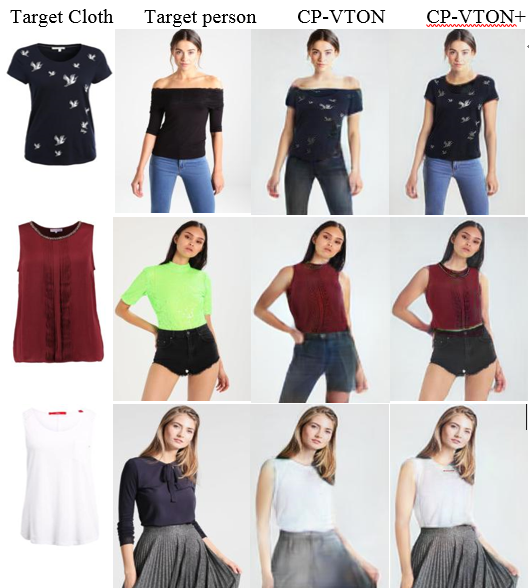
\includegraphics[height=8.5cm, scale=1]{figures/cpvton_cpvton+keyresult.png}   % TODO
\caption{The proposed VTON results}
\label{fig:cpvton_cpvton+keyresult}
\end{figure}

The key contribution of the papers are 3 ways: First, we provide the classified performance evaluations of existing Image-based algorithms. Second, the origins are the limitations and reason of seemingly well working of the existing algorithms are  identified. Third, the direct solutions are proposed to tackles the identified problems. The proposed method might be not the optimal way to solve the problem but it can explicitly show the level of effects of identified issues in the final results.


\section{Classified Performance Evaluation of Image-Based VTON}

\subsection{Image-based VTON}

In this Section, we started with evaluating the 2D image based VTON algorithms. We considered CP-VTON \cite{Wang2018TowardCI} published in 2018 as the benchmark algorithm. The previous and following in 2019 share same input image and information conditions with CP-VTON and compare the results with it. Here we include the SCM based-VTON, VITON\cite{Han2017VITONAI}, and  CP-VTON \cite{Wang2018TowardCI}, however, we believe the performance strength and weakness are similar in the other algorithms too.


The Image based VTON algorithms are mostly composed of two stages: (1) cloth warping step that warps the try-on cloth to align with the pose and shape of the target model (called GMM in CP-VTON: geometric Manipulation Module)\cite{Wang2018TowardCI}, and (2) blending step that blends the warped cloth onto the target human image (called TON in CP-VTON: Try-On Network)\cite{Wang2018TowardCI}. CP-VTON assumes the target human image is pre-processed for a cloth agnostic human representation by a human pose estimation like OpenPose\cite{Cao2018OpenPoseRM} and human parsing like LIP\cite{Liang2018LookIP}. The human representation is composed of 1) heat maps for each joints 2) silhouette of human body, and 3) face and skin pixels patches (non-cloth and human identity area). We use the same dataset collected by Han et al. used in VITON\cite{Han2017VITONAI} and CP-VTON\cite{Wang2018TowardCI} papers.
 

% Add some paper summary after CP-VTON .... and explain the differences from our works.

 
\subsection{Classification Rule}

First of all, as shown in Table 1, the criteria for classifying the experimental samples were divided into the degree of occlusion of the costume, the pose of the subject, and the complexity of the costume itself. The degree of obscuration is a factor that affects the accuracy of the object of deformation, the posture is the degree of deformation, and the complexity of the clothes means the processing complexity of the clothes themselves. However, it is included in the range of classification, but not included in the actual experiment is shown in parentheses. Excluded conditions are those that are not included in the test data or that the evaluation is considered to be complex in the current technology. Based on this, six cases were classified as follows.

\begin{itemize}

\item B: Little obscuration and posture (long sleeves, short arms)
\item OP: Same as S, but partly covered by hair and arms
\item OB: A large part of the clothing is covered by the bottoms.
\item OF: If the front of the clothing is covered by the arms (long sleeves, short sleeves)
\item P: If there is a large posture deformation (large movement of the arm or twisted or lateral posture)
\item S: When there is a large body shape change (all or part of the body is thick or pregnant)

\end{itemize}

For reference, the costume of the data used is a T-shirt (without a collar) or the like, and the costume is generally formed in a simple form. It is also worth noting that most clothing is limited, such as monochromatic or monotone patterns.


Although several to tens of images were used for each type of experiment, they are not included in the paper due to the relationship between pages. 5 and Fig. 6, only representative images are presented for explanation.

\begin{itemize}

\item Wearing the Same Costume

In the same clothing experiment, performance was compared based on IoU, SSIM and visual results.

\begin{itemize}

\item B: All three algorithms showed high performance for short arm costumes. In particular, SCMM showed high performance. However, for long arms, the deformation of the arm was not good. This seems to be because the matching and deformation are mainly based on the whole silhouette. VITON and CP-VTON show that they are synthesized by complementing some of them in the synthesis process. Including the skeletal information can be supplemented, but at present, no algorithm has been developed for automatically extracting the skeletal information of the garment.

\item OP: Partial obstruction caused by hair, etc., caused this part to be excluded from the scope of the purpose, and had some influence on the deformation of the clothes. VITON and CP-VITON also exhibited the same problem because they included head and skin in their representation. Therefore, it is expected to improve the GMM part by removing elements such as hair and using only body shapes.
\item OB: Occlusion due to bottoms occurs. SCMM algorithms do not distinguish between deformation and occlusion. Therefore, IoU shows a deterioration, and especially the long arm is reduced and the skin is lifted up. Since VITON and CP-VITON use body information rather than box body, this effect seems to be reduced.


\item OF: When the front part is covered by the arm, human expression can be used to distinguish the area of the clothes from the area of ??the arm. However, this part may not be clear during deep learning synthesis.

\item P: If there is a large pose change, all three algorithms have a big error in the clothing deformation. This is considered to be a big limitation using the two-dimensional algorithm.
\item S: In the case of the data of the same costume, the costume itself was largely prepared, so the error was not large.
\end{itemize}

\item Experiment with wearing a new costume
 
The wearing of a new outfit is, in effect, the ultimate result of the application. As above, objective evaluation would be possible, but at present, one model could not present dataset that has more than two costumes. Although limited, it is possible to compare the relative differences of each algorithm based on visual results.


\begin{itemize}

\item B: The clothing deformation itself shows good results similar to the result of the same costume, but there are some differences according to the algorithms in the synthesis. When switching from long to short arms, SCMM does not restore the skin color of the arm and VITON and CP-VTON seem to produce it. In particular, CP-VTON shows excellent generating ability. This is an advantage of using pix2pix-based deep learning over non-deep learning.
\item OP: The performance was similar to that of the same clothes.
\item OB: The same characteristics as the same image, that is, the SCMM showed a problem that can not distinguish between the mask and deformation.
\item OF: The same characteristics as the costume. Here too, in the case of SCMM, the synthesis algorithm needs to be improved when switching from short arm to long arm.
\item P: As in the case of the same costume, there was a large error in deformation.
\item S: It showed some adaptation to body shape change. In particular, VITON and CP-VTON have been shown to adapt very well to body shape changes.

\end{itemize}

In addition to the analysis of each condition in addition to the analysis of each condition, it can be seen that there are the following big features. First, it was confirmed that the shape change of clothes by GMM has an influence on the current wear clothes. The reason is that SCMM uses the area of the current costume, and deep learning methods use the body itself, but the area of the current costume is reflected in the correct answer mask used in the learning process.

\end{itemize}


 
\subsection{Analysis Summary}


Even though the success and failure cases are presented and compared with other algorithms' results, the failure case analysis is not enough for understanding the origin of failure cases and therefore difficult to find the solution for them. A classified evaluation would be better for this understanding. Here we summarized the classified results from our another study. We classify input try-on cloth and target human images according to the posture and body type of the person, the degree of occlusion of the clothes, and the characteristics of the clothes. Quality is compared in IoU for the warping step and in SSIM for the final blending step for same cloth re-try-on cases. We also tested for the new cloth try-on cases but did not include here for limitation of spaces, and the same cloth cases are enough to explain the tendencies of the performances. Though in general CP-VTON generates the best quality image, the relative comparison is not the main purpose of the analysis. Please refer to Figure \ref{fig:classified2DVTONresult} for detailed results.


\begin{figure}
\centering
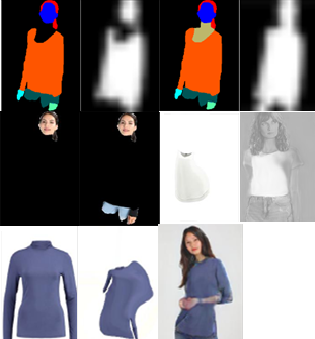
\includegraphics[height=8.5cm, scale=1]{figures/cpvtonissues.png}   % TODO
\caption{The issues in CP-VTON}
\label{fig:cpvtonissues}
\end{figure}


Firstly, the target try-on area is dependent upon current cloth shape. Especially, the neck area pixels are labeled as background and some body areas are occluded by hairs or accessories (Fig. 3 (a) left), which affects in cloth warping and blending. Secondly, all the unintended part, faces, bottom-clothes and legs have to be preserved in blending stage. But other parts except face and hair are missing in CP-VTON\cite{Wang2018TowardCI} human representation and generated at blending stage, which is all right for general synthesis application but not desirable in VTON application (Fig. 3 (b) left). Thirdly, the texture is often not vivid, which is due to the composition. Examining the original loss function of TON network, the term for the composition alpha mask are poorly formulated as simple regularization loss.   

\begin{equation}
L = c_1 | I_0-I_{GT} |+  c_2 L_{VGG}+c_3 |1-M_0 |        
\end{equation} 

Fourthly, since no label in the area of warped cloth is the same color as background, white colored clothes are confused and improperly processed in the blending stage (Fig. 3 (c))


Finally, GMM module using Spatial Transform Network\cite{JaderbergSZK15} with TPS (Thin Plate Spline)\cite{Bookstein1989PrincipalWT} deformation cannot handle strong 3D deformation due to the target pose and also generates artifacts because of the person representation inputs. For example, hands-up and folded arms.  Note that many errors in the warping stage are often hidden in the blending stage when the target clothes are single-colored, which can be expected in practical conditions 
%(Fig. 3 (d)).



%Especially note that the warped cloth are often too much different for desired shape. It is originated two facts. First the 3D deformation that any 2D deformation including non-rigid transform such as TPS is quite limited, especially any 2D deformation cannot handle when the two area in the original image are overlapped in the destination images. There for when the arms of long sleeved cloth occlude the main body, 2D warping cannot approximate the 3D deformation properly. Second, the deformation needs corresponding points  between the source nd target image. The cloth are extremely difficult object to find the corresponding points. The STN (spatial transform network)\cite{JaderbergSZK15} and SCM (shape context matching)\cite{BelongieMP02} cannot find the corresponding points when the target cloth and original cloth has different shapes. In conclusion, the 2D image based algorithm has serious limitation in the range of applications. It can apply to the mild posed target human only and simple short sleeved cloth, mainly because the inherent limitation of 2D deformation method including non-rigid ones, and the poor performance of matching algorithm.  To overcome this limitation, we consider to model the try-on cloth into 3D model and apply the 3D deformation

\begin{figure}
\centering
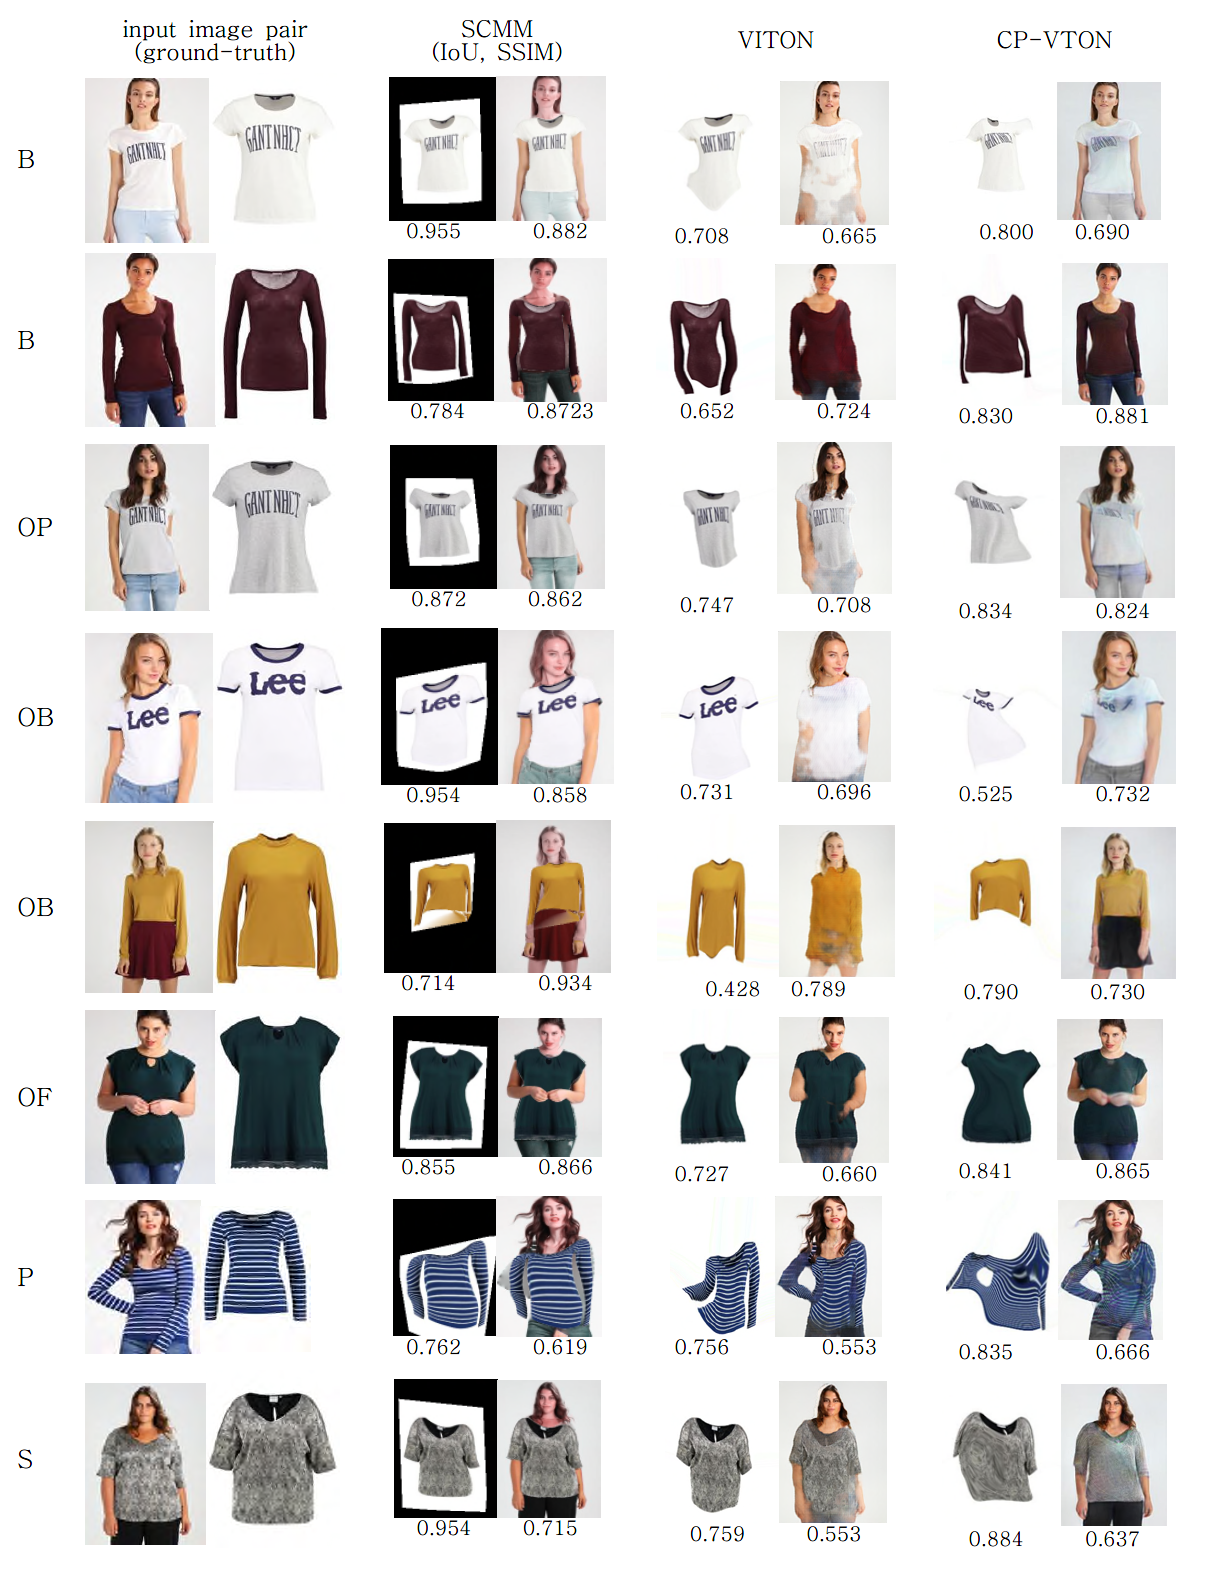
\includegraphics[height=13.5cm, scale=1]{figures/2dvton_same.png}   
\caption{Classified Evaluation of Image-based VTONs (same cloth re-try-on)}
\label{fig:2dvton_same}
\end{figure}

\begin{figure}
\centering
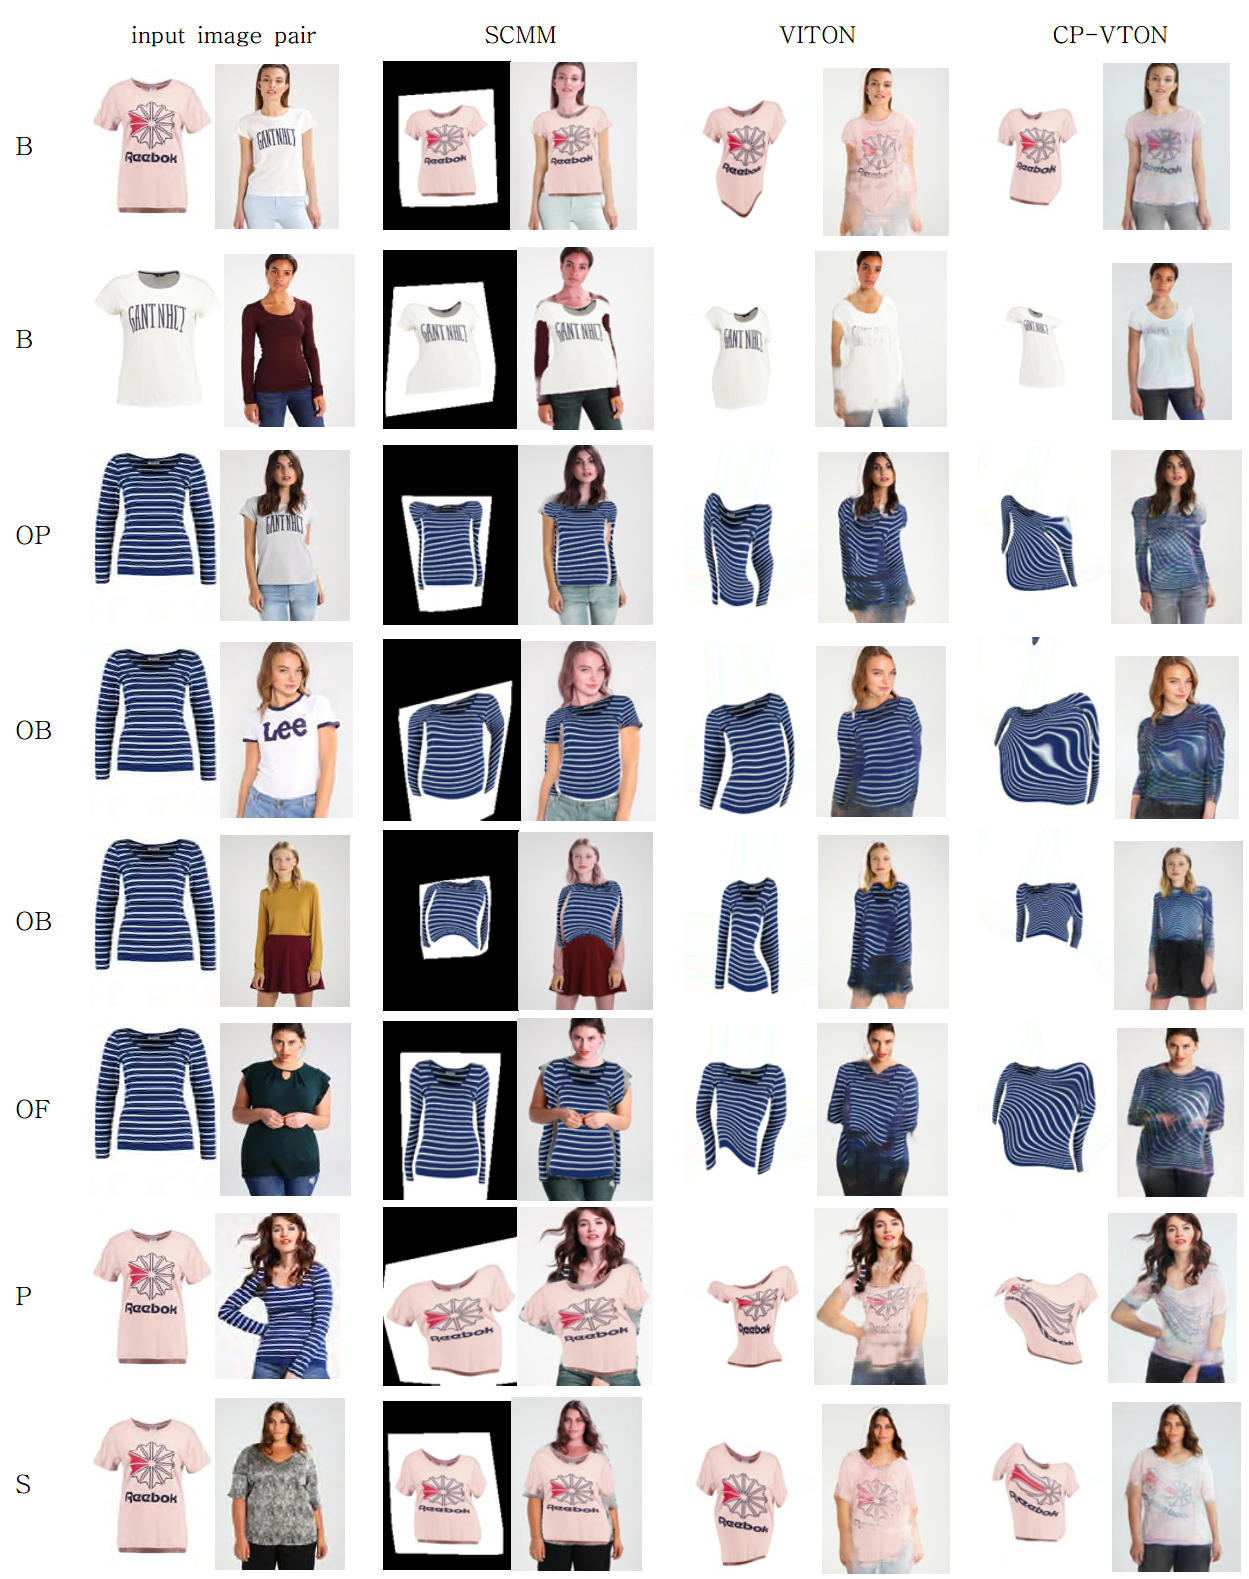
\includegraphics[height=13.5cm, scale=1]{figures/2dvton_diff.png}  %% TODO  
\caption{Classified Evaluation of Image-based VTONs (new cloth try-on)}
\label{fig:2dvton_diff}
\end{figure}


\section{CV-VTON+} \label{section:cpvton+}

\subsection{Overview} 

Fig. 4 illustrates the new pipeline emphasizing the modifications from CP-VTON, which tackles all 4 issues above mentioned except extreme 3D pose of target human.

\begin{itemize}

\item Correction on the cloth agnostic representation   


\begin{itemize}

\item Modification 1: We added a new label ‘Skin’ to the human parsing data to represent the human body shape more accurately (Fig. 2. (a) right).

\item Modification 2: We removed the hair label from the Reserved Regions of GMM’s Person Representation input, i.e. only face remains.  

\end{itemize}


\item Un-changed human area inclusion  

\begin{itemize}
\item Modification 3: We added extra human components except the target cloth area, e.g. bottom clothes and legs in the Reserved Regions of Person Representation to TOM, along with face and hair (Fig. 2. (b) right).

\end{itemize}

\item Improving Composition alpha-map 


\begin{itemize}

\item Modification 4: In the mask loss term in TOM loss function, we replaced the Composition Mask with supervised ground truth mask for a strong alpha mask.

\begin{equation}
L=c_1 |I_0-I_{GT} |+  c_2 L_{VGG}+c_1 |M_{GT}-M_0 |       
\end{equation}

\item Modification 5: Lastly, we added the binary mask of warped cloth to TOM network input so that TOM can clearly differentiate the target cloth area regardless of cloth color.  

\end{itemize}

\item GMM improvement Will be here: GIC loss and Mask ETC

TODO!!!

TODO!!!

TODO!!!

TODO!!!

TODO!!!

TODO!!!

TODO!!!

TODO!!!

TODO!!!






















\end{itemize}


\begin{figure}
\centering
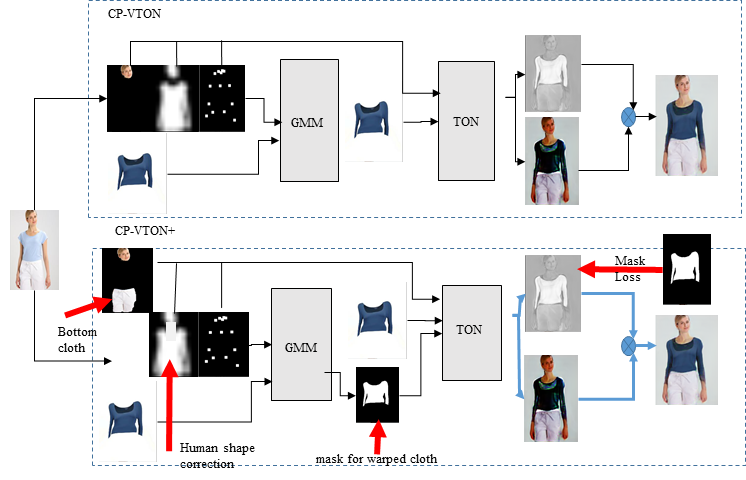
\includegraphics[height=6.5cm, scale=1]{figures/cpvton+pipeline.png}   
\caption{Comparison: CP-VTON and CP-VTON+}
\label{fig:piepline}
\end{figure}

\section{Experiment and Results} 

\subsection{Implementation details} 

We used the same dataset used in CP-VTON, collected first for VITON. We used IoU and SSIM performance metrics for the same cloth retry-on cases for GMM and TOM. For final output quality measures, we used SSIM, Inception Score (IS)[9] and LPIPS[10] for different cloth try-on. The subjective qualities can be examined in Fig. 5/7.  Special comments are required for the IoU values, where CP-VTON (0.78) is slightly higher than CP-VTON+ (0.75). The un-expected results originated due to CP-VTON generating as in the current cloth shape. However, similar clothes are not always applicable, furthermore, it generates wrong shaped results for different clothes. Fig. 6 illustrates this with two typical example, plugging and normal tops

\subsection{Comparative Results}

\begin{figure}
\centering
%\includegraphics[height=6.5cm, scale=1]{figures/vton_result1.png} 
%\includegraphics[height=6.5cm, scale=1]{figures/vton_result2.png} 
\caption{VTON results}
\label{fig:vtonresults}
\end{figure}


Final, i.e., TOM results are evaluated with non-reference methods, LPIPS[10], IS[9] and SSIM. Our proposed method, CP-VTON+ outperforms CP-VTON in LPIPS with 0.1263 against 0.1397, in SSIM with 0.8076 over 0.7798, and in IS with 2.76 over 2.7417. The subjective evaluation shows significant visual improvements, especially in cloth textures such as logos and patterns (Fig. 7). We added the test results for all test cases for comparison between CP-VTON and CP-VTON+ in supplementary materials, together with the categorized comparison of SCM-based VTON, VITON and CP-VTON.


\subsection{Ablation Study}

Figure ~\ref{fig:ablation} we highlight the impact of the identified problems and improvement of the proposed method step-by-step through the ablation study of CP-VTON+. The first and second columns are target humans and try-on clothes, respectively. The third column is vanilla CVP-VTON results. The fourth column is when unchanged clothes and body parts are added to the reserved region inputs of TOM, retaining the original pants texture. The fifth column is when the mask loss function of TOM is updated with the target cloth area, making the texture and color of cloth sharp and vivid. Finally the sixth and last column is when the body masks are updated, replacing the skin area wrongly labelled as background and hair are removed from the reserved region input of GMM, making GMM can better cloth-and-hair-agnostic human representation.  


WHEN WE GET the GMM improvement, Where we can add this? may be the first step?

\begin{figure}
\centering
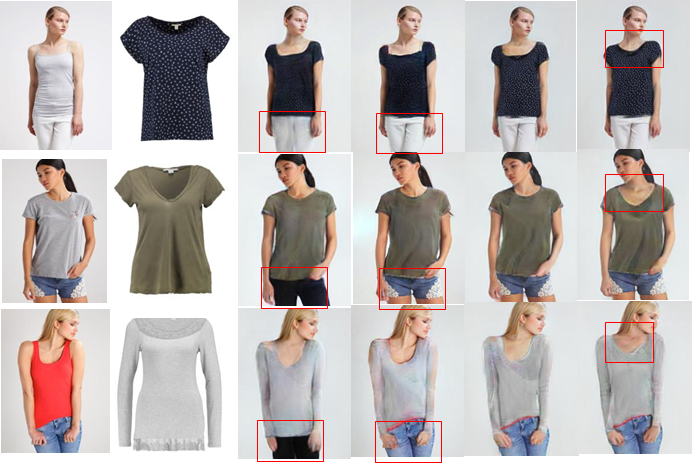
\includegraphics[height=6.5cm, scale=1]{figures/ablation.png} 
\caption{Ablation study of CP-VTON+. From left to right column. Target human, try-on cloth, CP-VTON, w. human representation, warped cloth mask and mask loss function updated, and CP-VTON+
}
\label{fig:ablation}
\end{figure}



\subsection{Known further issues}


Even though our modification  improve the VTON results a lot, and showing highly natural results, note that the dataset has limited samples for difficult cases, like the long sleeved, complicated shaped, or textured cloth and large posture target human. We amplify the key problems identified not try to list all the small problems. 

As Figure ~\ref{fig:gmmfailure} shows two typical failure cases due to the cloth warping. First row shows when the arms heavily covers the body area. The warped cloth does not match to the human body and TON failed in hiding the warping error. It is due to the limitation of STN (Spatial Transform Network). STN is originally developed for invert the (augmented) input images for different camera views and camera distortion. Non-rigid transforms, including TPS algorithms, cannot handle the strong 3D deformations of cloth.  Also the 3D poses induce self-occlusions. The TON network should recognized the cloth area and skin areas, like naked arms. One practical short-term solution would be to restrict the pose of target human image from the customer. And the long-term solution would be developed an 3D cloth deformation techniques for the GMM step, which is under studied by the authors. 

The second rows shows the another problems. Even without strong 3D posture of the target human, the warped cloth often shows un-realistic results. The accuracy for matching and warping of STN is not fully studied for VTON applications. 

%%%%%%%%
WE need to say something.
%%%%
    

The output image quality of all image-based VTON algorithms including ours depend upon the quality of input human representation, i.e., estimated joint locations and parsed human segmentation. The poses of target humans are usually (or forced) rather simple so that the state-of-the-art pose estimation algorithms can provide fairly accurate positions. However the quality of parsed human are not always good enough, especially when the target human wear complicated clothes. Also one can restrict the complexity of human images in pose and cloth style, but still the accuracy at the segmentation boundary sometimes affects the blended image results as shown in third row case in Fig ~\ref{fig:ablation}, where the pixels of the current top cloth, which is mislabelled as bottom cloth, remained in the blending result. There fore high quality human parsing algorithm especially around boundaries are required.   


\begin{figure}
\centering
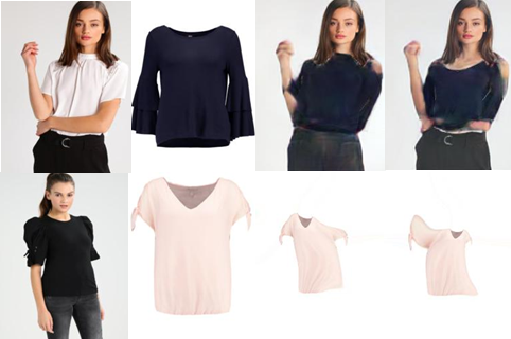
\includegraphics[height=6.5cm, scale=1]{figures/gmmfailure.png} 
\caption{Cloth Warping Failure of CP-VTON+. From left to right column. Target human, try-on cloth, CP-VTON, and CP-VTON+  (Why not same first and second ??)
}
\label{fig:gmmfailure}
\end{figure}
 
\section{Conclusions}

Almost all real computer vision algorithms have a certain condition where they work successfully and not. Therefore it is more important than merely developing better algorithms to identify the working condition of algorithms and approaches.  By categorized cloth and human inputs and analysis not only final try-on results but also intermediate results of the pipeline, e.g. the warped cloth, we showed the key successful and unsuccessful conditions and origins of a typical image-based VTON algorithm, CP-VTON. 

With these identified issues, a CP-VTON+, an improvement to CP-VTON was proposed, which produces significant quality improvements over existing state-of-the-art algorithm, CP-VTON. 

However, there remains several areas that we could not yet solved. The automatic warping to the target human shape is still challenging in feature point search and matching and limitation of non-rigid 2-D transforms, and the accuracy human parsing  needs to be improved.
  
     
\clearpage
% ---- Bibliography ----
%
% BibTeX users should specify bibliography style 'splncs04'.
% References will then be sorted and formatted in the correct style.
%
\bibliographystyle{splncs04}
\bibliography{cpvton+bib}



\end{document}
